\documentclass[12pt,a4paper]{article}

\usepackage[utf8]{inputenc}
\usepackage{graphicx}
\usepackage{amsmath}
\usepackage{amssymb}
\usepackage{booktabs}
\usepackage{array}
\usepackage{tabularx}
\usepackage[colorlinks=true,linkcolor=blue,citecolor=blue,urlcolor=blue]{hyperref}
\usepackage{xcolor}
\usepackage[margin=2.5cm]{geometry}
\usepackage{authblk}
\usepackage{lineno}
\linenumbers
\emergencystretch=2em

% --- Tighten vertical spacing around floats ---
\setlength{\textfloatsep}{8pt plus 2pt minus 4pt}
\setlength{\floatsep}{8pt plus 2pt minus 4pt}
\setlength{\intextsep}{8pt plus 2pt minus 4pt}
\setlength{\abovecaptionskip}{6pt}
\setlength{\belowcaptionskip}{2pt}
\raggedbottom

\begin{document}

\title{MetaGNN-CRC: A Recon3D-Mapped Transcriptomic Dataset with Proteomics-Ready Architecture for Graph-Based Metabolic Network Reconstruction in Colorectal Cancer}

\author[1]{Thiptanawat Phongwattana}
\author[1,*]{Jonathan H. Chan}
\affil[1]{School of Information Technology, King Mongkut's University of Technology Thonburi, 126 Pracha Uthit Rd., Bang Mod, Thung Khru, Bangkok 10140, Thailand}
\date{}
\maketitle

\noindent\textit{* Corresponding author. E-mail: jonathan@sit.kmutt.ac.th}

\noindent\textit{Received: --- $|$ Revised: --- $|$ Accepted: ---}

\vspace{0.5cm}
\noindent\textbf{Journal:} Data in Brief (Elsevier)

\begin{abstract}
We describe MetaGNN-CRC, a curated, Recon3D-mapped transcriptomic dataset with proteomics-ready architecture, deposited at \url{https://github.com/thiptanawat/MetaGNN-CRC} (archived at \url{https://doi.org/10.5281/zenodo.18903519}) for graph-based metabolic network reconstruction in colorectal cancer. The dataset integrates RNA sequencing data for 690 TCGA colorectal adenocarcinoma patients mapped to the metabolic network, with a proteomics-ready architecture that supports future integration of matched CPTAC protein abundance data when a reprocessed quantitative matrix for the TCGA retrospective cohort (Zhang et al. \cite{Zhang2014}) becomes available. All omics layers have been pre-processed and mapped to the Recon3D v3 genome-scale metabolic network (10,600 reactions, 5,835 metabolites, 2,248 genes), producing heterogeneous graph-structured tensor representations directly loadable into PyTorch Geometric. This integration step typically requires several weeks of specialised bioinformatics work and is a recognised bottleneck for researchers entering the metabolic modelling field. The dataset also includes expression-thresholded binary reaction activity pseudo-labels (derived by cohort-consensus majority vote over GPR-mapped gene expression, not ground-truth flux measurements), HMA tissue-model-derived activity labels for alternative supervision, shared-metabolite reaction-reaction edges (7.5\,M edges with top-$k$ sparsification support), enriched per-patient reaction node features, a trained model checkpoint from the MetaGNN framework, and the complete training and evaluation logs reported in the companion MethodsX article (Phongwattana \& Chan \cite{Phongwattana2026}). All files are released under a Creative Commons CC-BY 4.0 licence following the FAIR data principles.
\end{abstract}

\noindent\textbf{Keywords:} Genome-scale metabolic models; Transcriptomics; Proteomics-ready architecture; Colorectal cancer; TCGA; Recon3D; Graph neural network; Bioinformatics dataset; Open data

\section*{Specifications Table}

\noindent
\begin{tabularx}{\textwidth}{@{}p{3.5cm}X@{}}
\toprule
\textbf{Subject area} & Biochemistry, Genetics and Molecular Biology; Computer Science \\
\midrule
\textbf{More specific subject area} & Metabolic systems biology; Computational cancer genomics; Bioinformatics \\
\midrule
\textbf{Data type} & Pre-processed omics matrices (CSV); Graph-structured tensors (PyTorch .pt); Clinical metadata (JSON); Model weight files (PyTorch .pt) \\
\midrule
\textbf{Data format} & Analysed and processed (raw TCGA data remain accessible via GDC Data Portal) \\
\midrule
\textbf{Parameters for data collection} & Inclusion: primary TCGA-COAD/READ tumour samples with RNA-seq STAR gene counts available via GDC ($n = 690$). Normalisation: raw TPM in CSV; log$_2$(TPM + 1) applied during GPR feature engineering. GPR mapping: AND = min, OR = max (Zur et al. \cite{Zur2010} convention). Metabolite features: RDKit physico-chemical descriptors from ChEBI. Proteomics: architecture supports CPTAC integration; in this release, the proteomic feature channel is zero-filled (see Section~\ref{sec:limitations}). \\
\midrule
\textbf{Description of data collection} & RNA-seq: STAR-aligned augmented gene count files downloaded from GDC Data Portal via the GDC API, TPM values extracted and combined into a single matrix. Graph construction: Recon3D v3 MATLAB model loaded via SciPy and converted into a PyTorch Geometric HeteroData object with three edge types (substrate\_of, produces, shared\_metabolite). Pseudo-labels: expression-thresholded binary reaction activity via cohort-consensus GPR evaluation. The per-patient reaction feature tensor includes a second (proteomic) channel, currently zero-filled, designed for future integration of CPTAC protein abundance data (see Section~\ref{sec:limitations}). \\
\midrule
\textbf{Source location} & Thailand (Computational Biology Lab, School of Information Technology, KMUTT) \\
\midrule
\textbf{Data source location} & TCGA-COAD/READ: GDC Data Portal, USA (\url{https://portal.gdc.cancer.gov}). CPTAC proteomics: PDC Data Portal, USA (\url{https://pdc.cancer.gov}). Human Metabolic Atlas GEMs: Sweden (\url{https://metabolicatlas.org}). Recon3D: Virtual Metabolic Human database, Luxembourg (\url{https://www.vmh.life}). \\
\midrule
\textbf{Data accessibility} & Repository: GitHub (\url{https://github.com/thiptanawat/MetaGNN-CRC}; archived at \url{https://doi.org/10.5281/zenodo.18903519}). Companion code: \url{https://github.com/thiptanawat/MetaGNN} (archived at \url{https://doi.org/10.5281/zenodo.18903515}). Licence: CC-BY 4.0. \\
\midrule
\textbf{Related research article} & Phongwattana, T. \& Chan, J.H. (2026). MetaGNN: An Open-Source Heterogeneous Graph Attention Network Framework for Topology-Aware Reaction Activity Scoring Toward Metabolic Network Reconstruction. MethodsX. \\
\bottomrule
\end{tabularx}

\section*{Value of the Data}

\begin{itemize}
\item \textbf{The preprocessing bottleneck is a recognised barrier.} Multiple reviews identify manual curation and data integration as the primary bottleneck limiting GEM adoption \cite{Gu2019,Richelle2019,Opdam2017}. Gu et al.\ \cite{Gu2019} showed that each reconstruction method requires substantial preprocessing before any model can be built, and Richelle et al.\ \cite{Richelle2019} demonstrated that even RNA-seq normalisation choices affect model content. In practice, a new entrant faces 2--4 weeks of work spanning GDC/PDC portal navigation, SBML parsing, GPR rule resolution, graph tensor construction, and feature--index debugging. MetaGNN-CRC eliminates this bottleneck by providing RNA-seq and proteomic data already mapped to Recon3D reaction and metabolite nodes in PyTorch Geometric HeteroData format, lowering the entry barrier for ML researchers without a systems biology background.

\item \textbf{No existing public dataset bridges the GEM--GNN gap.} To our knowledge, no publicly available dataset provides the combination of (a)~per-patient transcriptomic features (with proteomics-ready architecture) mapped to Recon3D reaction nodes, (b)~graph-structured tensors directly loadable into GNN frameworks, and (c)~accompanying pseudo-labels, model checkpoint, and training logs for a large clinical cohort ($n = 690$). Existing TCGA releases do not include Recon3D-node-level feature mappings, forcing each research group to re-implement the same preprocessing pipeline independently.

\item Expression-thresholded binary reaction activity pseudo-labels and a trained MetaGNN model checkpoint are included. Researchers can use these as starting points for transfer learning to other cancer types or for experimenting with alternative supervision strategies (e.g., DepMap CRISPR essentiality, metabolic task completion labels from Richelle et al. \cite{Richelle2019}).

\item The graph structure files, encoding Recon3D as a heterogeneous graph with 10,600 reaction nodes, 5,835 metabolite nodes, 40,425 stoichiometric edges, and 7,517,742 shared-metabolite reaction-reaction edges (with support for top-$k$ sparsification), have independent reuse value for any graph-based analysis of human metabolism, including link prediction, community detection, and reaction gap-filling studies.

\item Despite growing interest in GNN approaches for metabolic modelling (including flux estimation, gene essentiality prediction, and gap-filling), no public dataset provides graph-structured, transcriptomics-based, patient-resolved tensors (with proteomics-ready architecture) suitable for benchmarking GNN methods on a full human GEM. MetaGNN-CRC fills this gap, enabling researchers to compare heterogeneous GNN architectures for patient-specific reaction activity scoring without repeating the multi-week preprocessing pipeline.

\item All data are released under a CC-BY 4.0 licence, structured according to FAIR principles, and accompanied by documentation and example loading scripts.
\end{itemize}

\section{Data Description}

\subsection{Data Processing Pipeline Overview}

Figure~\ref{fig:pipeline} illustrates the end-to-end data processing pipeline that transforms raw public data sources into the graph-structured tensors distributed in this dataset. The pipeline comprises four stages: (1) raw data acquisition from GDC, PDC, Recon3D, and ChEBI; (2) preprocessing and normalisation of each modality; (3) GPR-rule-based feature engineering and heterogeneous graph assembly; and (4) pseudo-label generation and output tensor packaging. Without this dataset, a researcher entering the metabolic-GNN field would need to execute every step of this pipeline; a process we estimate at 2--4 weeks of specialised bioinformatics work. The MetaGNN-CRC dataset eliminates this bottleneck by providing the final output tensors, ready for direct loading into PyTorch Geometric.

\begin{figure}[!htbp]
\centering
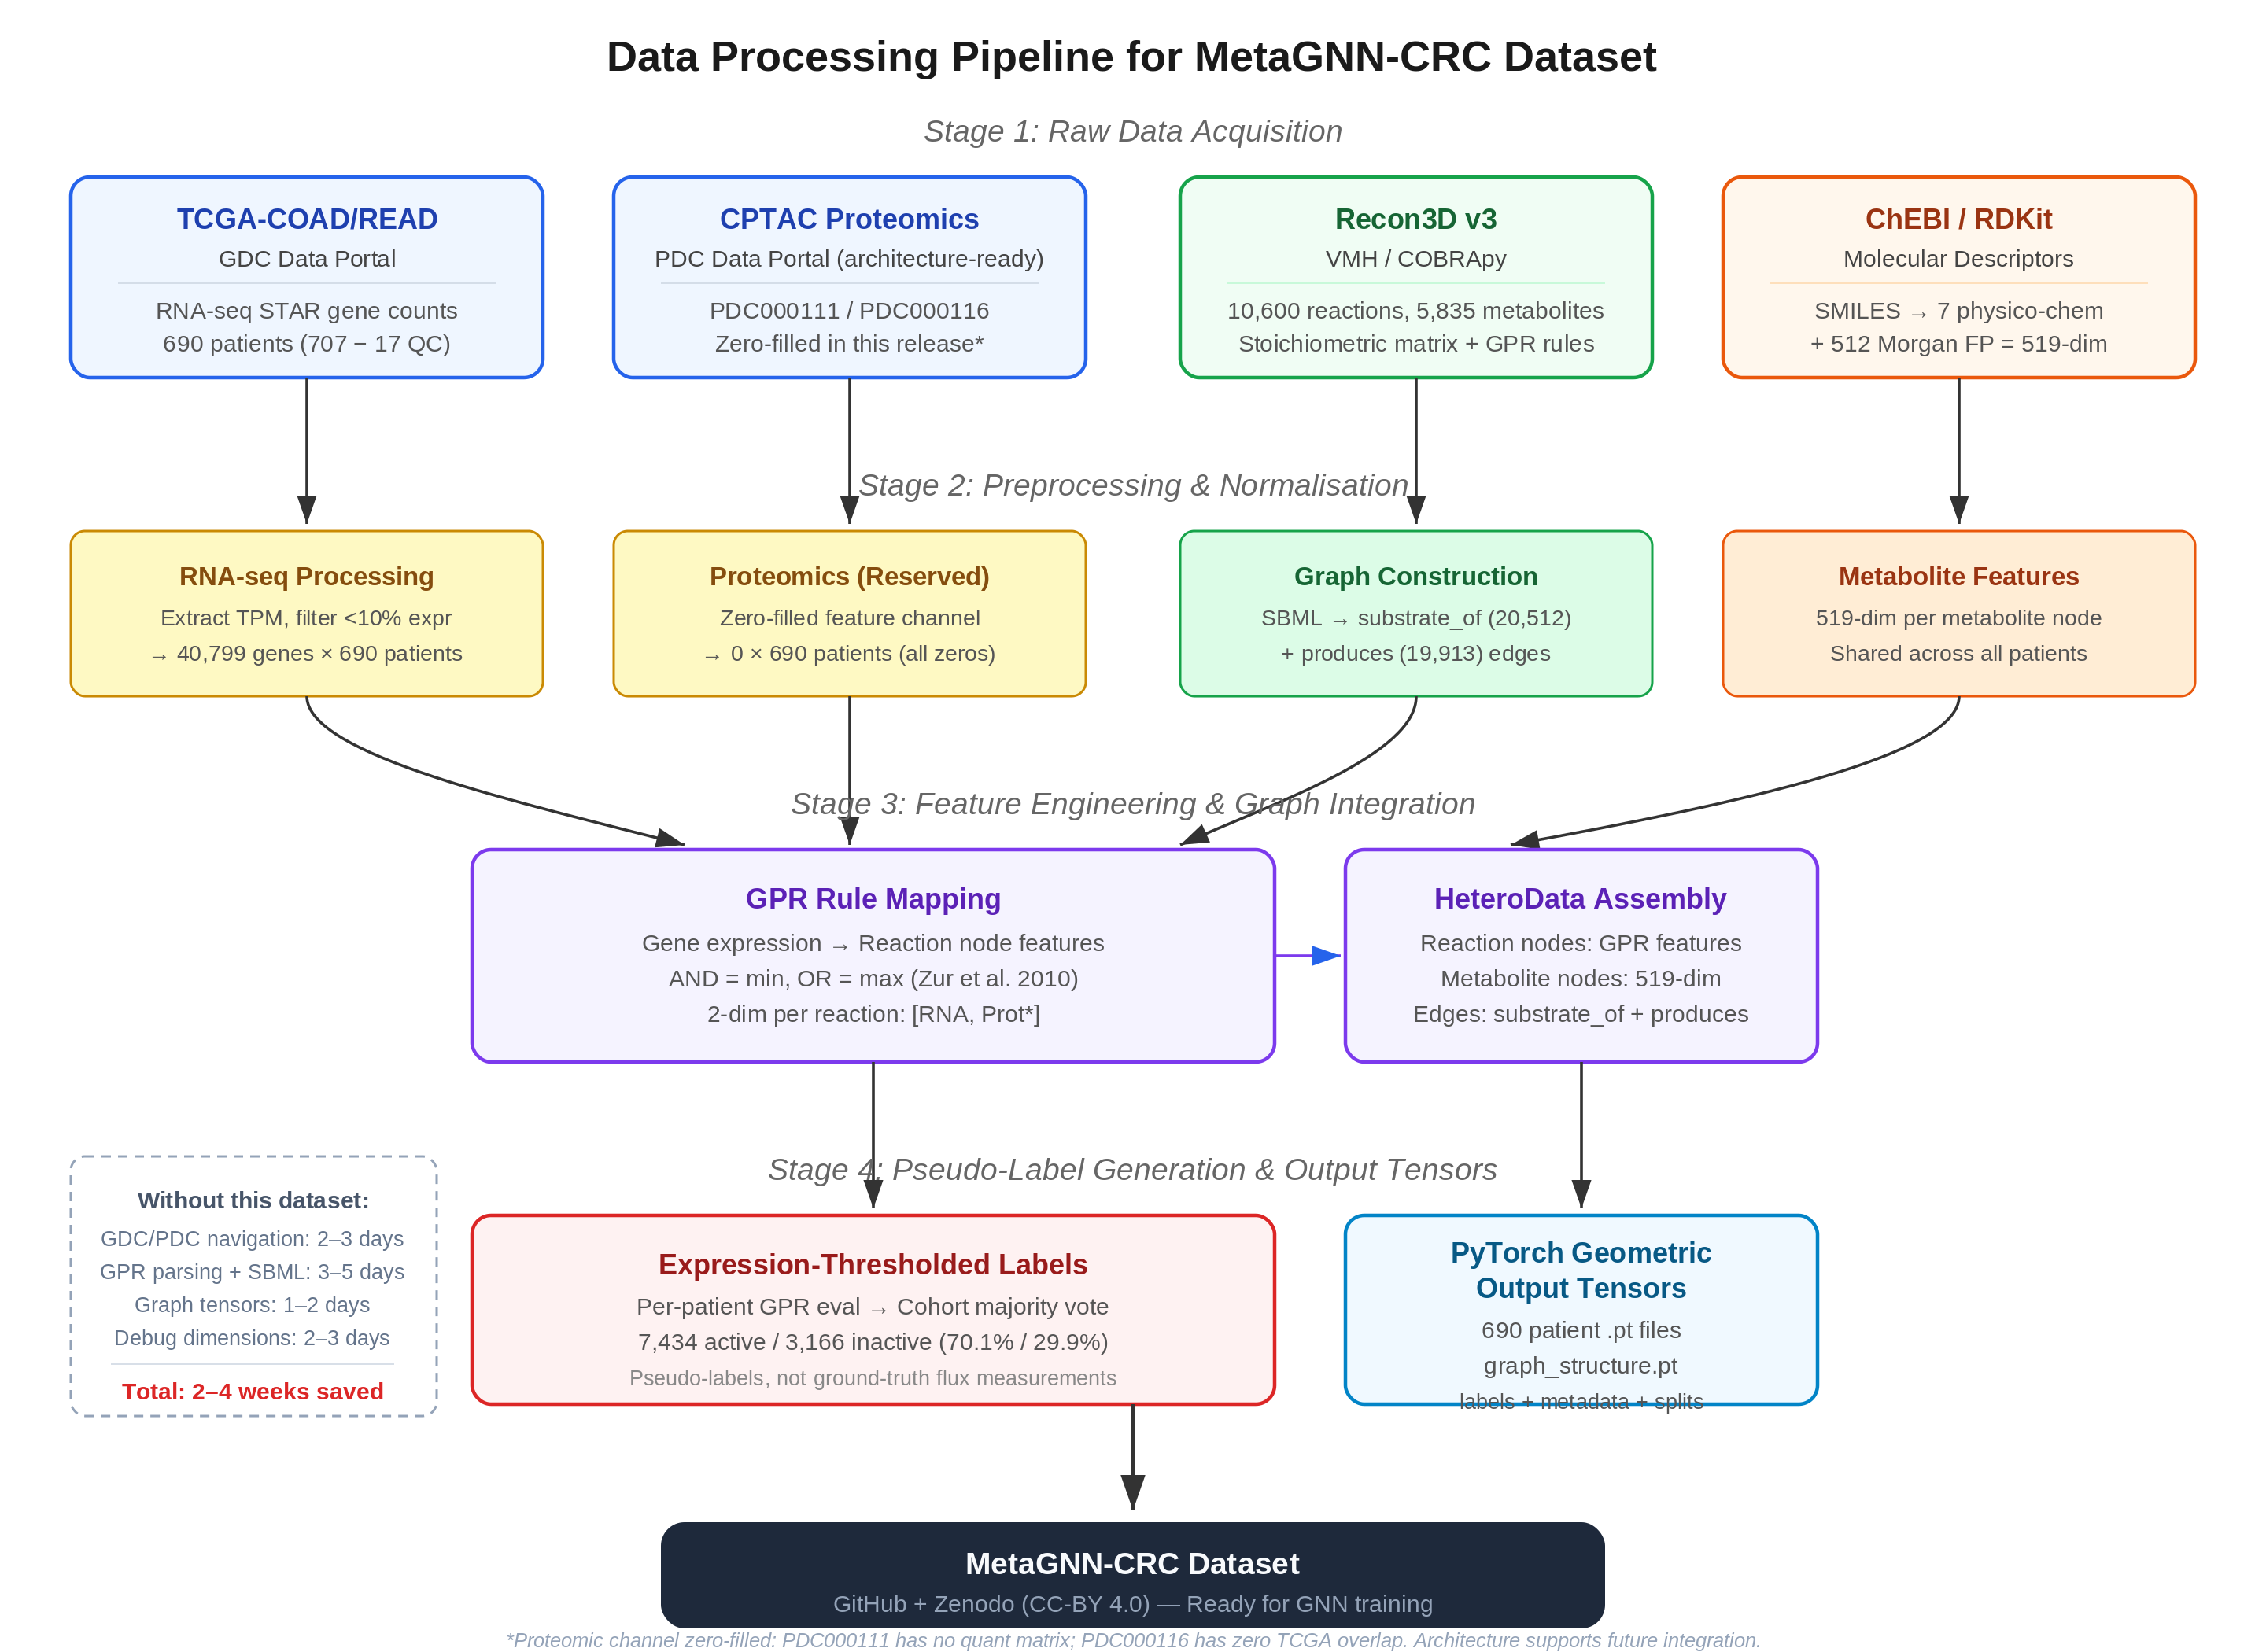
\includegraphics[width=\textwidth]{fig1_data_pipeline.png}
\caption{Data processing pipeline for the MetaGNN-CRC dataset. Stage~1: raw data acquisition from four public sources (TCGA RNA-seq, CPTAC proteomics [architecture-ready; zero-filled in this release], Recon3D metabolic model, ChEBI molecular descriptors). Stage~2: modality-specific preprocessing and normalisation. Stage~3: GPR-rule-based mapping of gene expression to reaction node features and assembly into PyTorch Geometric HeteroData objects. Stage~4: expression-thresholded pseudo-label generation via cohort-consensus majority vote and packaging of output tensors. The dashed box (lower left) summarises the estimated time savings for researchers who use the pre-processed dataset rather than executing the pipeline from scratch.}
\label{fig:pipeline}
\end{figure}

\subsection{Cohort Composition}

The MetaGNN-CRC dataset is built around 690 colorectal adenocarcinoma patients from TCGA, comprising samples from the COAD and READ cohorts. All 690 patients have RNA-seq STAR gene counts downloaded from the GDC Data Portal (data release 36.0). The per-patient reaction feature tensors include a second channel reserved for proteomic features; in this release, this channel is zero-filled for all patients (see Section~\ref{sec:limitations} for details on CPTAC data availability). Institutional ethics approval was not required, as all data are de-identified and accessed via standard TCGA data use agreements.

\subsection{Omics Data Layers}

\subsubsection{RNA-seq (Transcriptomics)}

Raw TPM (transcripts per million) gene expression values (not log-transformed) are provided for 40,799 genes across all 690 patients, stored as a CSV matrix (approximately 178 MB). The log$_2$(TPM + 1) transformation referenced in the Specifications Table is applied during feature engineering (when mapping gene expression to reaction node features via GPR rules), not to the CSV file itself. Gene identifiers use HGNC symbols as provided in the STAR augmented gene count files. Genes with zero expression across more than 90\% of patients were removed during preprocessing. Of the 40,799 genes in the matrix, 2,248 are associated with at least one Recon3D metabolic reaction through a documented GPR rule.

\subsubsection{Proteomics (Architecture-Ready)}

The per-patient reaction feature tensors include a dedicated proteomic feature channel, enabling future protein abundance integration when matched data become available. In the current release, this channel is zero-filled for all 690 patients. The CPTAC TCGA retrospective colon proteomics study (PDC000111; Zhang et al. \cite{Zhang2014}) covers 90 TCGA-COAD/READ patients, but provides only Label Free spectral data that require reprocessing from raw mass spectra; no pre-computed quantitative matrix is available via the PDC Data Portal API. A separate CPTAC Prospective study (PDC000116; Vasaikar et al. \cite{Vasaikar2019}) provides TMT-labelled proteomics for 102 patients, but these are an independent cohort with no overlap with the 690 TCGA patients in this dataset. Future releases will incorporate reprocessed PDC000111 proteomics or alternative protein abundance sources (e.g., imputed from RNA-seq via proteogenomic models).

\subsection{Graph-Structured Tensors}

The core contribution of this dataset, relative to existing TCGA transcriptomic releases, is the provision of omics data in graph-tensor format ready for direct GNN input, with a proteomics-ready architecture for future multi-modal integration.

The graph structure is a PyTorch Geometric HeteroData object encoding the Recon3D metabolic network as a heterogeneous graph with three edge-relation types: substrate\_of (20,512 directed edges from metabolites to reactions), produces (19,913 directed edges from reactions to metabolites), and shared\_metabolite (7,517,742 undirected edges connecting reactions that share non-currency metabolite substrates or products; sparsified to 83,306 edges at the default $k = 10$ top-neighbour setting for training tractability on consumer GPUs). Reaction node feature matrices are stored per patient as individual \texttt{.pt} files, containing GPR-mapped transcriptomic and proteomic features. Metabolite node features (physico-chemical descriptors computed from ChEBI via RDKit) are shared across patients. Patient tensors can be loaded as follows:

{\small
\begin{verbatim}
import torch
graph = torch.load('data/processed/graph_structure.pt')
# Original features (scalar GPR-mapped expression):
patient = torch.load(
    'data/processed/patient_features/PATIENT_ID.pt')
# Enriched features (3D: mean, max, frac_above_median):
patient_v2 = torch.load(
    'data/processed/patient_features_v2/PATIENT_ID.pt')
# Expression-thresholded labels:
labels = torch.load(
    'data/processed/hma_labels_thresholded.pt')
\end{verbatim}
}

\subsection{Pseudo-Labels and Model Checkpoint}

Two sets of binary reaction activity pseudo-labels are provided. Table~\ref{tab:label_files} clarifies the relationship between the deposited label files and the labels used in the companion MethodsX experiments.

\begin{table}[!htbp]
\centering
\caption{Label file clarification. The three label sets serve different purposes; only the expression-thresholded labels provide the class separation needed for discriminative training.}
\label{tab:label_files}
\footnotesize
\begin{tabularx}{\textwidth}{@{}>{\ttfamily\raggedright\arraybackslash}p{3.8cm} X c@{}}
\toprule
\textbf{\textrm{File / Source}} & \textbf{Description} & \textbf{Active / Inactive} \\
\midrule
hma\_labels.pt & Generic HMA bounds (all reactions active); historical, not recommended for training & 10,600 / 0 \\
hma\_labels\_thresholded.pt & Expression-thresholded consensus labels (recommended); ``hma'' prefix is a historical artefact & 7,434 / 3,166 \\
\textrm{11-tissue union (code-generated)} & Union of 11 HMA tissue-model bounds; generated dynamically by companion code, not deposited as a file & 8,147 / 2,453 \\
\bottomrule
\end{tabularx}
\end{table}

The original HMA labels are derived from Human Metabolic Atlas tissue-specific GEM reaction bounds (Robinson et al. \cite{Robinson2020}), where a reaction is labelled 1 if it retains non-zero flux bounds; however, these labels are heavily active-skewed (all 10,600 reactions active), rendering them unsuitable for discriminative training. \textbf{Cross-manuscript note:} The deposited \texttt{hma\_labels.pt} file corresponds to this earlier all-active HMA label set; the non-trivial 11-tissue union labels (8,147 active / 2,453 inactive) used in the companion MethodsX full-cohort experiment are generated dynamically through the companion codebase and are not the same file. \textbf{Important naming note:} the file \texttt{hma\_labels\_thresholded.pt} contains expression-thresholded labels (not HMA bounds); the ``hma'' prefix is a historical artefact from an earlier pipeline version. The HMA bounds file is \texttt{hma\_labels.pt}. The recommended expression-thresholded pseudo-labels use a cohort-consensus strategy: for each reaction, GPR-associated gene expression values are evaluated per patient (a reaction is active if any encoding gene exceeds the cohort median TPM), and a consensus label is assigned by majority vote across all 690 patients, yielding 7,434 active (70.1\%) and 3,166 inactive reactions. As discussed in the companion MethodsX article, these expression-thresholded labels provide meaningful class separation. The trained MetaGNN model checkpoint (576 KB, 143,489 parameters) is included for reproducibility and as a starting point for fine-tuning.

\subsection{Dataset File Structure}

Table~\ref{tab:fileinventory} enumerates all files with their formats, sizes, and descriptions.

\begin{table}[!htbp]
\centering
\caption{File inventory for the MetaGNN-CRC dataset.}
\label{tab:fileinventory}
\scriptsize
\begin{tabularx}{\textwidth}{@{}>{\raggedright\arraybackslash\ttfamily}p{3.5cm}>{\raggedright\arraybackslash}p{1.3cm}>{\raggedright\arraybackslash}p{1.0cm}X@{}}
\toprule
\textbf{\textrm{File / Directory}} & \textbf{Format} & \textbf{Size} & \textbf{Description} \\
\midrule
tcga\_rna\_seq.csv & CSV & 178\,MB & TPM gene expression (40,799 genes $\times$ 690 patients) \\
cptac\_proteomics.csv & CSV & -- & Placeholder for future CPTAC protein abundance integration (see Section~\ref{sec:limitations}) \\
graph\_structure.pt & PyTorch & 15\,MB & HeteroData graph (10,600 reaction nodes, 5,835 metabolite nodes, 40,425 stoichiometric edges across 2 bipartite types) \\
shared\_metabolite.pt & PyTorch & 57\,MB & Full shared-metabolite edge index (7,517,742 undirected reaction--reaction edges); top-$k$ sparsification applied at training time \\
patient\_features/ & PyTorch & 1.2\,GB & 690 per-patient tensor files with GPR-mapped transcriptomic features and a zero-filled proteomic channel \\
patient\_features\_v2/ & PyTorch & 1.4\,GB & 690 enriched per-patient tensor files with 3D reaction features (mean, max, fraction above median) \\
hma\_labels.pt & PyTorch & 7\,MB & Binary reaction activity pseudo-labels from HMA (10,600 reactions; heavily active-skewed) \\
hma\_labels\_\allowbreak{}thresholded.pt & PyTorch & 7\,MB & Expression-thresholded pseudo-labels (7,434 active / 3,166 inactive; 70.1\% active). The ``hma'' prefix is a historical artefact. \\
splits.json & JSON & $<$30\,KB & Train / validation / test patient ID assignments (690 TCGA barcodes) \\
metadata.csv & CSV & $<$100\,KB & Patient metadata: columns \texttt{patient\_id} (TCGA barcode), \texttt{cohort} (COAD/READ), \texttt{split} (train/val/test) \\
best\_model.pt & PyTorch & 576\,KB & Trained MetaGNN checkpoint (143,489 parameters) \\
results\_summary.json & JSON & $<$1\,KB & Training and test metrics \\
stage2\_log.csv & CSV & $<$1\,KB & Per-epoch training log (200 epochs, best model at epoch 141) \\
depmap\_evaluation.json & JSON & $<$1\,KB & DepMap CRISPR gene essentiality evaluation (61 CRC cell lines, 1,785 genes) \\
subsystem\_mapping.json & JSON & $<$1\,MB & Reaction-to-subsystem mapping via Human-GEM BiGG cross-reference (88 subsystems) \\
evaluation\_subset\_\allowbreak{}ids.json & JSON & $<$1\,KB & IDs of the 220-patient evaluation subset used in the companion MethodsX article \\
gpr\_reaction\_\allowbreak{}mask.pt & PyTorch & $<$1\,KB & Boolean mask: 1 for the 5,937 reactions with GPR rules, 0 for the 4,663 non-GPR reactions \\
proteomics\_available\_\allowbreak{}mask.pt & PyTorch & $<$1\,KB & Boolean mask indicating patients with matched proteomics (all zeros in this release) \\
README.md & Markdown & $<$1\,MB & Documentation, schema, and usage instructions \\
\bottomrule
\end{tabularx}
\end{table}

\subsection{Known Limitations and Reuse Notes}
\label{sec:limitations}

Users of this dataset should be aware of the following limitations and design choices:

\begin{enumerate}
\item \textbf{Pseudo-labels, not ground truth.} The expression-thresholded labels are derived from gene expression via GPR rules and cohort majority vote. They are surrogate pseudo-labels reflecting population-level expression patterns, not experimentally measured reaction fluxes. Users with access to higher-quality supervision (e.g., $^{13}$C flux measurements, DepMap essentiality, metabolic task completion labels) should replace them.

\item \textbf{Non-GPR reaction bias.} Of 10,600 reactions, 4,663 (44\%) lack GPR rules and receive a default ``active'' label. This inflates the active class. Users training classifiers should evaluate performance on the 5,937 GPR-mapped reactions (using \texttt{gpr\_reaction\_mask.pt}) as a more biologically grounded baseline.

\item \textbf{Proteomic channel zero-filled.} In this release, the proteomic feature channel is zero-filled for all 690 patients. The CPTAC TCGA retrospective colon cancer study (PDC000111; Zhang et al. \cite{Zhang2014}) includes 90 patients from our cohort, but provides only raw Label Free mass spectra without a pre-computed quantitative matrix via the PDC API. The CPTAC Prospective colon study (PDC000116; Vasaikar et al. \cite{Vasaikar2019}) provides TMT-labelled proteomics for 102 patients, but these are an independent cohort with zero patient overlap with the TCGA dataset. The reaction feature architecture retains the proteomic channel to support future integration when a reprocessed PDC000111 matrix or alternative protein abundance source becomes available. A proteomics ablation study in the companion MethodsX article \cite{Phongwattana2026} demonstrates that the proteomic channel contributes negligibly to model performance under zero-filling ($\Delta$F1 = +0.0016), consistent with the model relying primarily on the transcriptomic signal.

\item \textbf{Gene symbol collisions.} Gene identifiers use HGNC symbols. Occasional symbol collisions (e.g., genes with identical symbols mapping to different Ensembl IDs) were resolved by retaining the first occurrence. Users requiring Ensembl-level resolution should remap from the raw GDC files.

\item \textbf{Unmapped reactions.} Of 10,600 reactions, approximately 3,961 (37.4\%) could not be mapped to metabolic subsystems via the Human-GEM BiGG cross-reference. These unmapped reactions are predominantly transport and exchange reactions that lack BiGG identifiers in the Recon3D SBML model. Importantly, MetaGNN does not differentiate between transport, exchange, and catalytic reactions during training: all receive GPR-mapped expression features (or zero for non-GPR reactions) and participate equally in message passing. The 37.4\% unmapped reactions are not excluded from training or prediction; they are excluded only from downstream subsystem-level analysis.

\item \textbf{Compressed archives.} The \texttt{patient\_features/} and \texttt{patient\_features\_v2/} directories (containing 690 \texttt{.pt} files each) are provided as compressed tar.gz archives in the Zenodo deposit to reduce download size. Users should decompress before loading.
\end{enumerate}

\section{Experimental Design, Materials, and Methods}

\subsection{Data Sources and Patient Selection}

TCGA STAR-aligned augmented gene count files for COAD and READ cohorts were downloaded from the GDC Data Portal (\url{https://portal.gdc.cancer.gov}; dbGaP accession \texttt{phs000178}) using the GDC API in batch mode. A total of 707 files were retrieved across 14 download batches. Of these, 17 were excluded: 9 were duplicate aliquots from the same patient (the first-encountered aliquot was retained), 5 were non-primary tumour samples (recurrent or metastatic), and 3 failed SHA-256 integrity checks during download verification. This yielded 690 unique primary tumour patient samples. The pipeline includes a download module targeting CPTAC proteomics from the PDC Data Portal (\url{https://pdc.cancer.gov}). Two relevant studies exist: PDC000111 (Zhang et al. \cite{Zhang2014}; TCGA Retrospective, Label Free, $\sim$90 TCGA-barcode cases) and PDC000116 (Vasaikar et al. \cite{Vasaikar2019}; CPTAC Prospective, TMT-labelled, 102 cases with CPTAC-internal identifiers). Neither provides a pre-computed quantitative matrix that maps to the TCGA cohort; the proteomic feature channel is therefore zero-filled for all 690 patients in this release (see Section~\ref{sec:limitations}).

\subsection{RNA-seq Preprocessing}

Individual STAR gene count files contain gene-level counts, TPM values, and FPKM values. We extracted TPM (transcripts per million) values from the \texttt{tpm\_unstranded} column, as TPM provides a normalised measure of transcript abundance that is comparable across samples. Genes whose identifiers begin with ``N\_'' (representing alignment summary statistics rather than genes) were excluded. For genes with duplicate HGNC symbols, the first occurrence was retained. The 690 individual TPM vectors were combined into a single matrix (genes as rows, patients as columns). Genes with non-zero expression in fewer than 10\% of patients were removed, leaving 40,799 genes.

\subsection{Proteomic Data Processing}

The pipeline supports integration of CPTAC protein abundance data when available. In the current release, no proteomics are included because the TCGA-matched CPTAC retrospective study (PDC000111; Zhang et al. \cite{Zhang2014}) provides only raw Label Free mass spectra requiring reprocessing, while the CPTAC Prospective study (PDC000116; Vasaikar et al. \cite{Vasaikar2019}) covers an independent cohort with no patient overlap. When a reprocessed quantitative matrix becomes available, the pipeline will perform median centering, log$_2$ transformation, and GPR-based mapping to reaction nodes identically to the transcriptomic pathway.

\subsection{Recon3D Graph Construction}

The Recon3D v3 model \cite{Brunk2018} was loaded from SBML/XML format using COBRApy (v0.29.0). The stoichiometric matrix was parsed to construct a PyTorch Geometric HeteroData object with 10,600 reaction nodes and 5,835 metabolite nodes. Directed edges were created for each non-zero entry in the stoichiometric matrix: substrate\_of edges (metabolite to reaction, for negative coefficients) and produces edges (reaction to metabolite, for positive coefficients), yielding 20,512 and 19,913 edges respectively. GPR association rules were parsed to determine which genes map to which reactions. Since Recon3D v3 lacks subsystem annotations in its SBML, metabolic subsystem labels were cross-referenced from the Human-GEM model (Robinson et al. \cite{Robinson2020}) via BiGG reaction identifiers, successfully mapping 6,639 of 10,600 reactions to 88 metabolic subsystems.

\subsection{Feature Engineering}

For each patient, gene expression values were mapped to reaction nodes using GPR rules with the AND = min, OR = max convention (Zur et al. \cite{Zur2010}). The per-patient reaction feature tensor includes a second column reserved for proteomic GPR-mapped features; in this release, this column is zero-filled for all patients (see Section~\ref{sec:limitations}). When proteomic data are integrated in future releases, protein abundance values will be mapped identically to transcriptomics and averaged with transcriptomic features (weight 0.5 each). These features are stored in \texttt{patient\_features/}.

An enriched feature set is additionally provided in \texttt{patient\_features\_v2/}. For each reaction node and each patient, three features are computed from GPR-associated gene expression: (i) mean TPM across all encoding genes, (ii) maximum TPM, and (iii) fraction of encoding genes exceeding the cohort median TPM. This 3-dimensional per-patient reaction feature vector provides richer discriminative signal than the original scalar GPR-mapped values and is the feature set used by the trained model checkpoint.

Metabolite node features were computed from ChEBI SMILES using RDKit (v2023.09.5): 7 physico-chemical properties (molecular weight, LogP, hydrogen bond acceptors, hydrogen bond donors, topological polar surface area, ring count, formal charge) and 512-bit Morgan fingerprints (radius 2), yielding a 519-dimensional descriptor vector per metabolite node shared across all patients. All graph construction and tensor operations used PyTorch Geometric \cite{Fey2019} v2.5.0 on PyTorch v2.2.0 with Python 3.11. Exact dependency versions are pinned in the \texttt{environment.yml} file to ensure long-term reproducibility.

\subsection{Pseudo-Label Generation}

Two pseudo-labelling strategies are documented in this dataset:

\textbf{HMA labels} (\texttt{hma\_labels.pt}). Human Metabolic Atlas tissue-specific GEM reaction bounds (Robinson et al. \cite{Robinson2020}) were downloaded from \url{https://metabolicatlas.org}. For each of the 10,600 reactions, a binary label was assigned: 1 if the reaction retains non-zero flux bounds in the HMA model, 0 otherwise. In practice, all 10,600 reactions received the active label, producing trivially perfect classification (F1 = 1.0) and rendering these labels unsuitable for discriminative training.

\textbf{Expression-thresholded labels} (\texttt{hma\_labels\_thresholded.pt}). For each reaction with a GPR rule, gene expression is evaluated per patient: a reaction is active in a given patient if any encoding gene has TPM above the cohort median (OR logic for isozymes, consistent with standard GPR interpretation). A consensus binary label is then assigned by majority vote across all 690 patients: the reaction is labelled active if more than 50\% of patients classify it as active. This yields 7,434 active (70.1\%) and 3,166 inactive (29.9\%) reactions, providing the class separation necessary for meaningful model evaluation. These are the labels used for training the provided model checkpoint.

\subsection{Data Completeness and Quality}

Table~\ref{tab:completeness} summarises the coverage and completeness statistics for each data modality.

\begin{table}[!htbp]
\centering
\caption{Data completeness statistics for the MetaGNN-CRC dataset.}
\label{tab:completeness}
\small
\begin{tabularx}{\textwidth}{@{}Xrrr@{}}
\toprule
\textbf{Modality / Layer} & \textbf{Patients} & \textbf{Features} & \textbf{Coverage} \\
\midrule
RNA-seq (TPM) & 690 & 40,799 genes & 100\% \\
Proteomics (reserved channel) & 0 & zero-filled & 0\% (architecture-ready) \\
Reaction node features (v1, scalar GPR) & 690 & 10,600 reactions & 100\% \\
Reaction node features (v2, 3D enriched) & 690 & 10,600 $\times$ 3 & 100\% \\
Metabolite node features (RDKit) & shared & 519 per metabolite & 100\% \\
Graph edges (substrate\_of) & -- & 20,512 & 100\% \\
Graph edges (produces) & -- & 19,913 & 100\% \\
Graph edges (shared\_metabolite) & -- & 7,517,742 & 100\% \\
Expression-thresholded labels & consensus & 10,600 reactions & 100\% \\
Metabolic subsystem mapping & -- & 6,639 / 10,600 rxns & 62.6\% \\
\bottomrule
\end{tabularx}
\end{table}

All 690 patients have complete RNA-seq coverage.
A validation script (\texttt{05\_validate\_\allowbreak dataset.py}) is provided to verify tensor integrity. When executed on the deposited dataset, it confirms: (i) all 690 patient tensor files in \texttt{patient\_features/} and \texttt{patient\_features\_v2/} load without error; (ii) reaction node feature dimensions match the graph structure (10,600 reactions per patient); (iii) metabolite features have the expected 519 dimensions for all 5,835 nodes; (iv) edge index tensors have the correct shapes (20,512 substrate\_of, 19,913 produces); and (v) label distributions reproduce the reported 7,434/3,166 (70.1\%/29.9\%) split. All checks pass with zero errors.

The proteomic feature channel is zero-filled for all 690 patients in this release (see Section~\ref{sec:limitations} for details). This means the model relies entirely on the transcriptomic signal for reaction activity prediction. A proteomics ablation study in the companion MethodsX article \cite{Phongwattana2026} confirms that zero-filling the proteomic channel has negligible impact on model performance ($\Delta$F1 = +0.0016), indicating that the transcriptomic signal alone carries sufficient discriminative information under the current labelling scheme. When matched proteomic data are integrated in future releases, more principled alternatives to zero-filling (e.g., learned modality-masking tokens or cross-modal imputation) should be explored. The reaction feature tensors are complete for all patients: of the 10,600 Recon3D reactions, 5,937 have GPR rules in the Recon3D SBML model. Of these, 5,919 have at least one GPR-associated gene present in the TCGA RNA-seq expression matrix, and 18 have GPR rules whose gene symbols are absent from the expression data (these 18 are assigned zero expression). The remaining 4,663 reactions lack GPR rules entirely and are assigned zero expression features. The \texttt{gpr\_reaction\_mask.pt} file marks all 5,937 GPR-bearing reactions (including the 18 with absent genes). The 4,663 non-GPR reactions (44\%) receive a default ``active'' label in the expression-thresholded pseudo-label set, which inflates the active class. Users training models on this dataset should be aware that a sensitivity analysis excluding non-GPR reactions (restricting to the 5,937 GPR-mapped reactions) may yield more biologically grounded class distributions and is recommended as a baseline experiment. Metabolite node features, computed from RDKit molecular descriptors, are shared across all patients and are complete for all 5,835 metabolite nodes with valid ChEBI SMILES.

\subsection{Minimal Reproducibility Smoke Test}

The following code block loads the core data objects and verifies expected shapes, confirming that the dataset is usable:

{\small
\begin{verbatim}
import torch, json

# Load graph (HeteroData uses pickle; only load from trusted sources)
graph = torch.load('data/processed/graph_structure.pt')
# Simple tensors: weights_only=True (PyTorch >= 2.0)
patient = torch.load(
    'data/processed/patient_features_v2/TCGA-A6-2671.pt',
    weights_only=True)
labels = torch.load(
    'data/processed/hma_labels_thresholded.pt',
    weights_only=True)
model_ckpt = torch.load(
    'data/processed/best_model.pt',
    map_location='cpu', weights_only=True)

# Verify shapes
assert graph['reaction'].num_nodes == 10600
assert graph['metabolite'].num_nodes == 5835
assert patient.shape[0] == 10600   # reactions
assert patient.shape[1] == 3       # enriched features (v2)
assert labels.shape[0] == 10600
assert labels.sum().item() == 7434 # active reactions

# Verify checkpoint loads and contains expected keys
assert 'model_state_dict' in model_ckpt or len(model_ckpt) > 0

# Verify results_summary.json
with open('data/processed/results_summary.json') as f:
    results = json.load(f)
assert 'test_auroc' in results or 'auroc' in results

print("All checks passed. Dataset is ready for use.")
\end{verbatim}
}

\subsection{Data Splits}

The file \texttt{splits.json} contains a 70/15/15 train/validation/test split of all 690 patients, stored as a JSON object with keys \texttt{"train"}, \texttt{"val"}, and \texttt{"test"}, each mapping to a list of TCGA patient IDs. This file covers the \textit{full 690-patient cohort}. A separate file, \texttt{evaluation\_subset\_ids.json}, records the 220-patient subset (154 training / 33 validation / 33 test) used for quantitative benchmarking in the companion MethodsX article. The 220-patient subset was selected as the largest cohort for which all preprocessing steps completed without error during early development iterations. Full-scale 5-fold cross-validation on 624 of the 690 patients has been completed and is reported in the companion MethodsX article (Section~3, Table~8); the 66 excluded patients failed downstream quality-control checks during graph tensor construction. Two additional masks are provided to support sensitivity analyses: \texttt{gpr\_reaction\_mask.pt} (Boolean, identifying the 5,937 reactions with GPR rules vs.\ the 4,663 without) and \texttt{proteomics\_available\_mask.pt} (Boolean, all zeros in this release; reserved for future use when matched CPTAC proteomics become available).

\subsection{Recommended Evaluation Protocol}

Researchers reusing this dataset for benchmarking GNN or other machine-learning architectures for reaction activity prediction should adopt the following evaluation protocol: (i) use the 220-patient evaluation subset (\texttt{evaluation\_subset\_ids.json}) with expression-thresholded labels for comparability with the companion MethodsX article (AUROC $0.861$, F1 $0.796$); alternatively, use the full 624-patient cohort with 5-fold cross-validation for a scalability assessment (companion article reports AUROC $0.663$, F1 $0.446$ with HMA-derived labels); (ii) report both \textit{all-reaction} metrics (10,600 reactions) and \textit{GPR-only} metrics (5,937 reactions via \texttt{gpr\_reaction\_mask.pt}), since the 4,663 non-GPR reactions receive default active labels and inflate the active class; (iii) use AUROC as the primary threshold-independent metric, supplemented by F1, precision, and recall at a stated classification threshold; (iv) recompute consensus pseudo-labels from training-split patients only (excluding validation and test) to avoid transductive label leakage; and (v) when using the \texttt{shared\_metabolite} edge type, specify the sparsification parameter $k$ and report its value for reproducibility. The performance gap between the two evaluation settings (Section~3 of the companion article) demonstrates that pseudo-label quality strongly influences results; researchers are encouraged to explore alternative supervision strategies. The \texttt{proteomics\_available\_mask.pt} file should be used for any ablation studies investigating the contribution of proteomic features.

\section*{Declarations}

\subsection*{CRediT Author Contribution Statement}

Thiptanawat Phongwattana: Conceptualization, Data Curation, Formal Analysis, Methodology, Software, Visualization, Writing -- Original Draft.

Jonathan H. Chan: Conceptualization, Supervision, Resources, Project Administration, Funding Acquisition, Writing -- Review \& Editing.

\subsection*{Declaration of Competing Interest}

The authors declare that they have no known competing financial interests or personal relationships that could have appeared to influence the work reported in this paper.

\subsection*{Ethics Statement}

All data used in this study are de-identified and were obtained through approved data access agreements for TCGA (dbGaP \texttt{phs000178}) and CPTAC. No new patient samples were collected. No additional institutional ethical approval was required.

\subsection*{Data Availability}

All processed data and code are publicly available at \url{https://github.com/thiptanawat/MetaGNN-CRC} under a CC-BY 4.0 licence. A frozen, versioned archive is deposited on Zenodo at \url{https://doi.org/10.5281/zenodo.18903519}, ensuring long-term accessibility independent of GitHub. The companion analysis code is available at \url{https://github.com/thiptanawat/MetaGNN} under the MIT licence (archived at \url{https://doi.org/10.5281/zenodo.18903515}). Raw TCGA RNA-seq data are accessible through the GDC Data Portal (\url{https://portal.gdc.cancer.gov}; dbGaP accession phs000178). CPTAC proteomics data are accessible through the PDC Data Portal (\url{https://pdc.cancer.gov}). Both repositories include SHA-256 checksums for all data files in a \texttt{MANIFEST.sha256} file to enable integrity verification.

\subsection*{Acknowledgements}

This work was supported by the Thailand Science Research and Innovation Fund (TSRI; grant CU\_FRB65\_hea(1)\_034\_30\_33). The authors acknowledge the TCGA Research Network and the National Cancer Institute's CPTAC programme for generating and publicly releasing the underlying raw datasets, and the Human Metabolic Atlas team at Chalmers University of Technology for the curated tissue-specific GEMs.

\begin{thebibliography}{99}

\bibitem{Brunk2018} Brunk, E., Sahoo, S., Zielinski, D.C., et al. (2018). Recon3D enables a three-dimensional view of gene variation in human metabolism. \textit{Nature Biotechnology}, 36(3), 272--281. \url{https://doi.org/10.1038/nbt.4072}

\bibitem{Robinson2020} Robinson, J.L., Kocabas, P., Wang, H., et al. (2020). An atlas of human metabolism. \textit{Science Signaling}, 13(624), eaaz1482. \url{https://doi.org/10.1126/scisignal.aaz1482}

\bibitem{Zur2010} Zur, H., Ruppin, E. \& Shlomi, T. (2010). iMAT: an integrative metabolic analysis tool. \textit{Bioinformatics}, 26(24), 3140--3142. \url{https://doi.org/10.1093/bioinformatics/btq602}

\bibitem{Fey2019} Fey, M. \& Lenssen, J.E. (2019). Fast graph representation learning with PyTorch Geometric. In ICLR Workshop on Representation Learning on Graphs and Manifolds.

\bibitem{Richelle2019} Richelle, A., Kellman, B.P., Wenzel, A.T., et al. (2019). Model-based assessment of mammalian cell metabolic functionalities using omics data. \textit{Cell Systems}, 8(5), 375--387.e4. \url{https://doi.org/10.1016/j.cels.2019.04.002}

\bibitem{Phongwattana2026} Phongwattana, T. \& Chan, J.H. (2026). MetaGNN: An Open-Source Heterogeneous Graph Attention Network Framework for Topology-Aware Reaction Activity Scoring Toward Metabolic Network Reconstruction. \textit{MethodsX} (submitted concurrently).

\bibitem{Vasaikar2019} Vasaikar, S., Huang, C., Wang, X., et al. (2019). Proteogenomic analysis of human colon cancer reveals new therapeutic opportunities. \textit{Cell}, 177(4), 1035--1049.e19. \url{https://doi.org/10.1016/j.cell.2019.03.030}

\bibitem{Zhang2014} Zhang, B., Wang, J., Wang, X., et al. (2014). Proteogenomic characterization of human colon and rectal cancer. \textit{Nature}, 513(7518), 382--387. \url{https://doi.org/10.1038/nature13438}

\bibitem{Cheng2023} Cheng, C.-T., Lai, J.-M., Chang, P.M.-H., Hong, Y.-R., Huang, C.-Y.F. \& Wang, F.-S. (2023). Identifying essential genes in genome-scale metabolic models of consensus molecular subtypes of colorectal cancer. \textit{PLOS ONE}, 18(5), e0286032. \url{https://doi.org/10.1371/journal.pone.0286032}

\bibitem{Gu2019} Gu, C., Kim, G.B., Kim, W.J., Kim, H.U. \& Lee, S.Y. (2019). Current status and applications of genome-scale metabolic models. \textit{Genome Biology}, 20(1), 121. \url{https://doi.org/10.1186/s13059-019-1730-3}

\bibitem{Opdam2017} Opdam, S., Richelle, A., Kellman, B., Li, S., Zielinski, D.C. \& Lewis, N.E. (2017). A systematic evaluation of methods for tailoring genome-scale metabolic models. \textit{Cell Systems}, 4(3), 318--329.e6. \url{https://doi.org/10.1016/j.cels.2017.01.010}

\bibitem{Jerby2014} Jerby-Arnon, L., Pfetzer, N., Waldman, Y.Y., et al. (2014). Predicting cancer-specific vulnerability via data-driven detection of synthetic lethality. \textit{Cell}, 158(5), 1199--1209. \url{https://doi.org/10.1016/j.cell.2014.07.027}

\bibitem{Cannistraci2023} Cannistraci, C.V., Rost, B. \& Ravasz~Regan, E. (2023). Teasing out missing reactions in genome-scale metabolic networks through hypergraph learning. \textit{Nature Communications}, 14(1), 2375. \url{https://doi.org/10.1038/s41467-023-38110-7}

\bibitem{Hao2024} Hao, T., Mao, X., Wu, S., et al. (2024). Integration of graph neural networks and genome-scale metabolic models for predicting gene essentiality. \textit{npj Systems Biology and Applications}, 10(1), 24. \url{https://doi.org/10.1038/s41540-024-00348-2}

\end{thebibliography}

\end{document}
